\documentclass[aspectratio=1610, english]{beamer} 
\usepackage{babel}
\makeatletter
\@ifclasswith{beamer}{polish}{
	\usepackage{polski}
}

\graphicspath{{static/}} 
\makeatother
\usepackage[utf8x]{inputenc}
\usepackage{physics}

\newcommand{\hzz}{ H\rightarrow ZZ^{*}\rightarrow 4 \ell}

\mode<beamer>{ 	% In the 'beamer' mode
	\hypersetup{pdfpagemode=FullScreen}         % Enable Full screen mode
	\usetheme[parttitle=rightfooter]{AGH}       % Show part title in right footer
	%\usetheme[nosidebar]{AGH}                  % Do not show sidebar on non-title slides
	%\usetheme[nosidebar, margins=1em]{AGH}     % Do not show sidebar on non-title slides and set both margins (left / right) to 1em
}
\mode<handout>{	% In the 'handout' mode
	\hypersetup{pdfpagemode=None}		
	\usepackage{pgfpages}
	\pgfpagesuselayout{4 on 1}[a4paper,border shrink=5mm,landscape]	% Show 4 slides on 1 page
	\pgfpageslogicalpageoptions{1}{border code=\pgfusepath{stroke}}
	\pgfpageslogicalpageoptions{2}{border code=\pgfusepath{stroke}}
	\pgfpageslogicalpageoptions{3}{border code=\pgfusepath{stroke}}
	\pgfpageslogicalpageoptions{4}{border code=\pgfusepath{stroke}}
  	\usetheme{boxes}
  	\addheadbox{structure}{\quad\insertpart\hfill\insertsection\hfill\insertsubsection\qquad}          % Content of header
 	\addfootbox{structure}{\quad\insertshortauthor\hfill\insertframenumber\hfill\insertsubtitle\qquad} % Content of footer
}

\AtBeginPart{ % At begin part: display its name
	\frame{\partpage}
} 
\author[Aleksandra Poreba, Aleksandra Kukielka]{Aleksandra Poreba, Aleksandra Kukielka}
\date{}

	\title[The $H \rightarrow ZZ^{*}$ decay analysis]{The case of Higgs boson production in $H \rightarrow ZZ^{*}$ decay}
	\subtitle{Introduction to the Particle Physics Data Analysis}

%%%%%%%%%%%%%%%%%
\begin{document}
\maketitle

%%%%%%%%%%%%%%%%
\begin{frame}{Outline}
	\tableofcontents
\end{frame}

%%%%%%%%%%%%%%%%%%%%%%%
\section{Physics motivation}

\begin{frame}
\frametitle{Physics motivation}
The physics motivation for the measurement:
\begin{itemize}
\item a good test for the SM,
\item a measurement of inclusive and differential fiducial cross sections,
\item tests of the spin and parity of the Higgs boson,
\item test of perturbative QCD calculations.
\end{itemize}

\end{frame}

\begin{frame}
\frametitle{The Feynman diagram}

\begin{figure} [H]
\centering
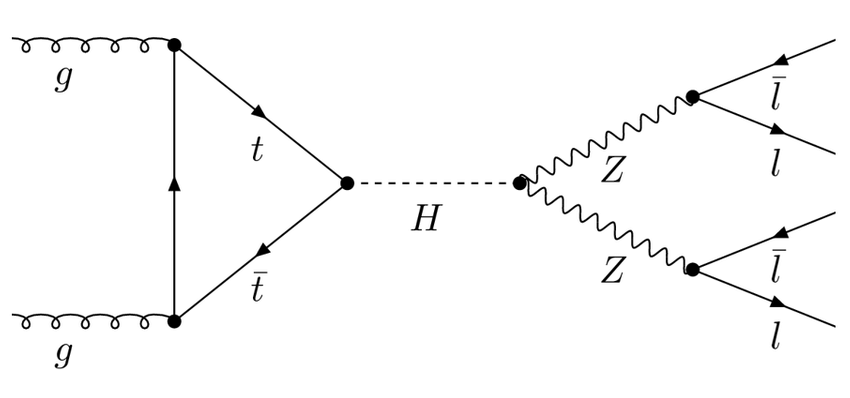
\includegraphics[width=8cm]{feynman_diagram.png}
\caption{Feynman diagram for $\hzz$ decay \cite{diagram}. }
\end{figure}

\end{frame}

%%%%%%%%%%%%%%%%%%%%%%%
\section{Event selection}

\begin{frame}
\frametitle{Event selection}
The final event-selection criteria for $ZZ^*$ production:

\begin{itemize}
\item single-electron or single-muon trigger satisfied,
\item exactly four leptons (electrons or muons) with $p_T>25, 15, 10, 7 GeV$, respectively,
\item Higgs-boson candidates are formed by selecting two $SFOS$ lepton pairs,
\item the leading pair is defined as the $SFOS$ \footnote{$SFOS$ - Same Flavour, Opposite Charge} pair with the mass $m_{\ell \ell, 1}$ closest to the $Z$ boson mass $m_Z$, and the subleading pair is defined as the SFOS pair with the mass $m_{\ell \ell, 1}$ second closest to $m_Z$. \cite{opendata}

\end{itemize}

\end{frame}

\begin{frame}
\frametitle{Cutflow Histogram}

\begin{figure} [H]
\centering
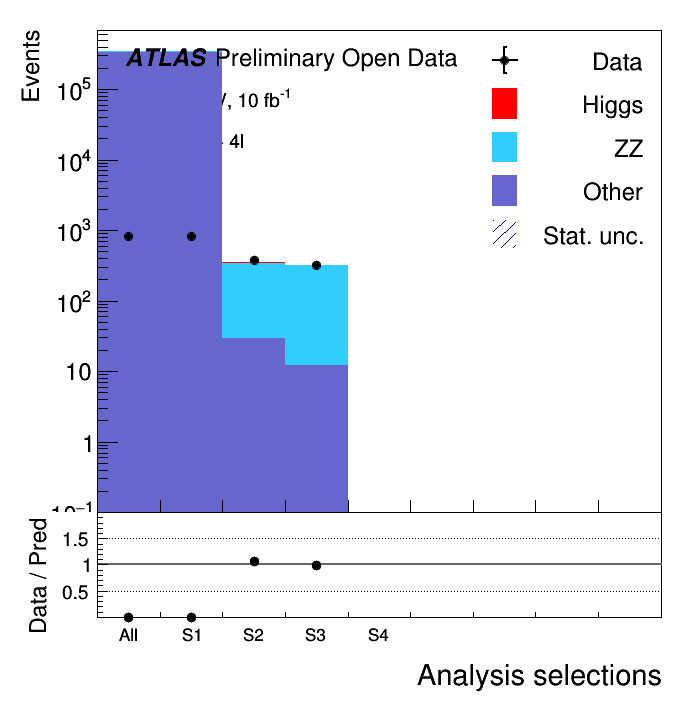
\includegraphics[width=6cm]{hist_cutflow.png}
\caption{The cutflow histogram: $S1$ - single-electron or single-muon trigger satisfied, $S2$ - four leptons with $p_T>25, 15, 10, 7 GeV$, $S3$ - two SFOS lepton pairs. }
\end{figure}

\end{frame}

%%%%%%%%%%%%%%%%%%%%%%%
\section{Expected number of events}

\begin{frame}
\frametitle{Expected number of events}
Expected number of events equals:
\begin{equation}
N^{ \hzz }=\sigma^{ \hzz }_{incl} \cdot L_{int},
\end{equation}
where:
\begin{description}
\item[$\sigma^{ \hzz }_{incl}$] = 3,62 $fb^{-1}$,
\item[$L_{int}$] = 10,06 $fb^{-1}$.
\end{description}
\vspace{1cm}
\begin{equation}
N^{ \hzz }=3,62 \: \mathrm{fb} \cdot 10,06 \: \mathrm{fb}^{-1} = 36,42.
\end{equation}

\end{frame}

%%%%%%%%%%%%%%%%%%%%%%%
\section{Background contributions}
\begin{frame}
\frametitle{Background contributions}
Processes constituting background of our analysis:
\begin{itemize}
\item non-resonant SM ZZ* production,
\item $t\bar{t}$ production,
\item Z+jets production.
\end{itemize}

\end{frame}

%%%%%%%%%%%%%%%%%%%%%%%
\section{Control plots}

\begin{frame}
\frametitle{Number of Leptons}

\begin{figure} [H]
\centering
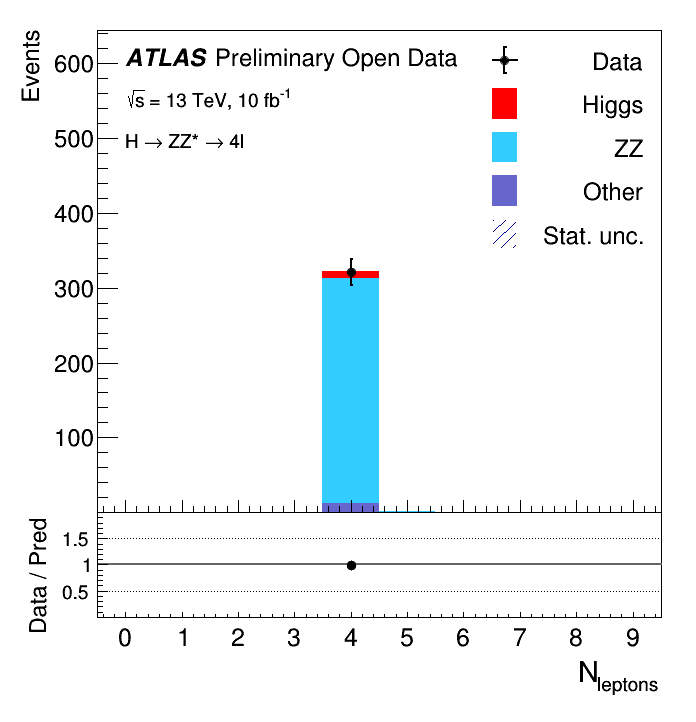
\includegraphics[width=6cm]{hist_n_leptons.png}
\caption{The histogram with number of leptons. }
\end{figure}

\end{frame}

%%%%%%%%%%%%%%%%%%%%%%%
\section{Cross-section measurement}
\begin{frame}
\frametitle{Cross-section measurement}
Cross-section of $\hzz$ was calculated using the following formula:
\begin{equation}
\sigma^{\hzz}=\frac{N_{data}-N_{bkg}}{C\cdot L_{int}}=\frac{N_{obs}}{C\cdot L_{int}} ,
\end{equation}
where:
\begin{description}
\item[$N_{data}$] - number of all events in data; $N_{data}=321$,
\item[$N_{bkg}$] - nubmer of background events; $N_{bkg}=315$,
\item[$N_{obs}$] - number of observed $\hzz$; $N_{obs}=6$,
\item[$C$] - correction factor; $C=0.525$,
\item[$L_{int}$] - integrated luminosity; $L_{int}=10.06 \: \mathrm{fb}^{-1}$.
\end{description}
\vspace{1cm}
\begin{equation}
\sigma^{\hzz}=\frac{321-315}{0.525\cdot 10.06}=\frac{6}}{0.525\cdot 10.06}=1,136 \: [\mathrm{fb}]
\end{equation}

\end{frame}
%%%%%%%%%%%%%%%%%%%%%%%
\section{Ideas for possible measurements}

%%%%%%%%%%%%%%%%%%%%%%%
\section{Bibliography}
%%%%%%%%%%%%%%%%%%%%%%%
\begin{frame}[allowframebreaks]{Bibliography}
	\begin{thebibliography}{9}
		\setbeamertemplate{bibliography item}[article]
		\bibitem{opendata}
			{The ATLAS collaboration\newblock Review of the 13 TeV ATLAS Open Data release \newblock \url{https://cds.cern.ch/record/2707171}}
		\bibitem{hzz}
			{Aaboud, Morad and others \newblock Measurement of inclusive and differential cross sections in the $ \hzz $ decay channel in pp collisions at $s√ = 13 TeV$ with the ATLAS detector \newblock \url{http://dx.doi.org/10.1007/JHEP10(2017)132}}
		\bibitem{diagram}
			{Passon, Oliver \newblock On the interpretation of Feynman diagrams, or, did the LHC experiments observe the Higgs to gamma gamma decay?}
	\end{thebibliography}
\end{frame}
\end{document}
